\documentclass[twocolumn, oneside,a4paper,10pt]{article}
\usepackage[english,brazilian]{babel}
\usepackage[alf]{abntex2cite}
\usepackage[utf8]{inputenc}
\usepackage[T1]{fontenc}
\usepackage[top=5mm, bottom=5mm, left=5mm, right=5mm]{geometry}
\usepackage{framed}
\usepackage{booktabs}
\usepackage{color}
\usepackage{hyperref}
\usepackage{graphicx}
\usepackage{float}
\graphicspath{{./Figuras/}}    
\usepackage{multicol}
\definecolor{shadecolor}{rgb}{0.8,0.8,0.8}

\newcommand{\EREM}{EREM Regina Pacis}
\newcommand{\curso}{\textbf{3 EMSI}}
\newcommand{\professor}{Prof. Leandro Vieira}

\begin{document}
\pagestyle{empty}
análise de gráficos

\begin{center}
\EREM
\par %pula uma linha
\curso
\par
\professor
\par
\LARGE \textbf{Atividade de Matemática}
\end{center}

\begin{enumerate}

\item No gráfico a seguir é mostra as médias de 4 estudantes de uma turma do 2º ano de uma turma do ensino médio em matemática, durantes 4 unidades do ano de 2020: I, II, III e IV:

\begin{figure}[h]
\center
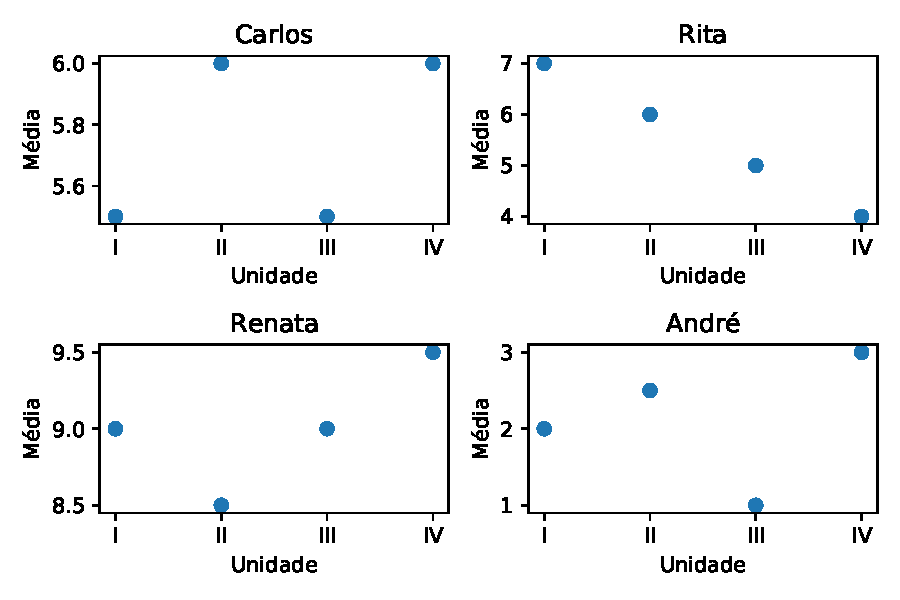
\includegraphics[width=10cm]{Figuras/01}
\end{figure}

\noindent Com base nas informações do gráfico responda às seguintes perguntas

	\begin{enumerate}
	\item Quem teve a maior média na unidade III?
	\item Sabendo que nessa escola a média é 6,5, quais estudantes ficaram abaixo da média na unidade II:
	\item Qual a média anual do estudante André?
	\item Quem teve a menor note na unidade IV?
	\end{enumerate}


\end{enumerate}

\flushbottom 
\flushright
"A arte de viver é simplesmente a arte de conviver...\\Simplesmente, disse eu? Mas como é difícil!\\(Mario Quintana)

\end{document}